\chapter{Bibliographie}
\label{cp:bibliographie}

\section{IMU}

\paragraph{Un IMU (Inertial Measurement Unit) est un dispositif électronique qui mesure et rapporte les données d'accélération linéaire, de vitesse angulaire et d'orientation d'un objet. Les IMU sont largement utilisés dans les applications de navigation inertielle, de robotique et de réalité virtuelle.}

\paragraph{Les IMU sont généralement composés de trois capteurs principaux : un accéléromètre, un gyroscope et un magnétomètre. L'accéléromètre mesure l'accélération linéaire de l'objet, le gyroscope mesure la vitesse angulaire de l'objet et le magnétomètre mesure le champ magnétique terrestre pour déterminer l'orientation de l'objet.}

\paragraph{Les IMU sont souvent utilisés en combinaison avec d'autres capteurs, tels que les GPS et les caméras, pour fournir des données de localisation et d'orientation plus précises. Les IMU sont également utilisés dans les applications de réalité virtuelle pour suivre les mouvements de la tête de l'utilisateur et fournir une expérience immersive.}

\begin{figure}[!htpb]
    \centering
    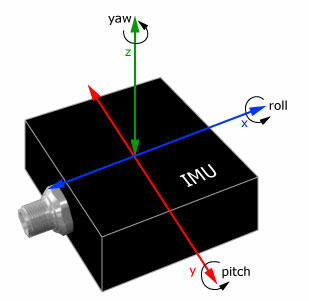
\includegraphics[width=0.5\linewidth]{Figures/imu.jpg}
    \caption[Schéma d'un IMU]{Schéma d'un IMU.}
    \label{fig:imu}
\end{figure}

\subsection{MPU6050}

\paragraph{Le MPU6050 est un IMU à 6 axes qui combine un accéléromètre et un gyroscope dans un seul boîtier. Le MPU6050 est largement utilisé dans les applications de robotique et de contrôle de mouvement en raison de sa petite taille, de sa faible consommation d'énergie et de sa précision élevée. Le MPU6050 est capable de mesurer l'accélération linéaire dans les trois axes et la vitesse angulaire dans les trois axes. Il utilise comme protocole de communication l'I2C.}

\begin{figure}[!htpb]
    \centering
    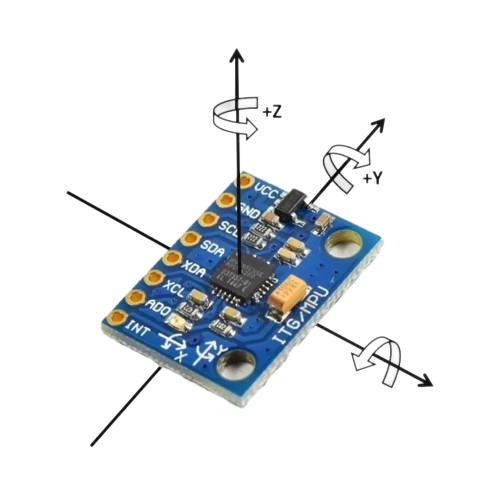
\includegraphics[width=0.8\linewidth]{Figures/mpu6050.png}
    \caption[Module MPU6050]{Module MPU6050.}
    \label{fig:mpu-6050}
\end{figure}


\subsection{I2C}

\paragraph{L'I2C (Inter-Integrated Circuit) est un bus de communication série d'architecture Maitre-esclaves qui permet à plusieurs périphériques de communiquer entre eux à l'aide d'un seul bus de données. L'I2C est largement utilisé dans les applications de capteurs et de contrôleurs pour connecter plusieurs périphériques à un microcontrôleur.}

\paragraph{L'I2C utilise deux fils pour la communication : un fil de données (SDA) et un fil d'horloge (SCL). Chaque périphérique connecté au bus I2C possède une adresse unique qui lui permet de communiquer avec les autres périphériques sur le bus. L'I2C prend en charge plusieurs vitesses de communication, allant de 100 kHz à 3,4 MHz.}

\begin{figure}[!htpb]
	\centering
	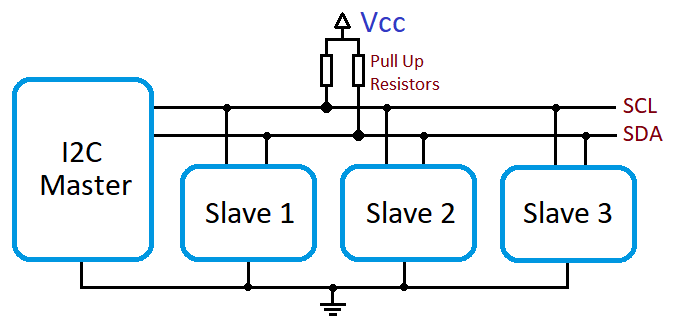
\includegraphics[width=\linewidth]{Figures/i2c.png}
	\caption[Schéma d'un bus I2C]{Schéma d'un bus I2C.}
	\label{fig:i2c}
\end{figure}

\subsection{Paquet I2C}

\paragraph{Un paquet I2C est composé de :}

\begin{enumerate}
	\item \textbf{Condition de demarage :} Un signal de valeur haute sur SDA et SCL indique le début de la communication.
	\item \textbf{Adresse client :} L'adresse du périphérique esclave auquel le maître souhaite communiquer.
	\item \textbf{Ecriture/Lecture :} Un bit de lecture/écriture indique si le maître souhaite lire ou écrire des données. (R = 1, W = 0)
	\item \textbf{Acknowledge :} Un bit de valeur basse sur SDA indique que le périphérique esclave a reçu les données avec succès.
	\item \textbf{Données :} Les données à écrire ou lire.
	\item \textbf{Acknowledge :} Un bit de valeur basse sur SDA indique que le périphérique esclave a reçu les données avec succès.
	\item \textbf{Condition d'arrêt :} Un signal de valeur basse sur SDA et haute sur SCL indique la fin de la communication.
\end{enumerate}

\paragraph*{\textbf{Adresse client} est composé de 7 bits d'adresse et d'un bit de lecture/écriture. Alors que \textbf{les paquets de données} peuvent etre sequentiels composés de 8 bits de données et un bit d'acknowledge entre eux.}

\begin{figure}[!htpb]
	\centering
	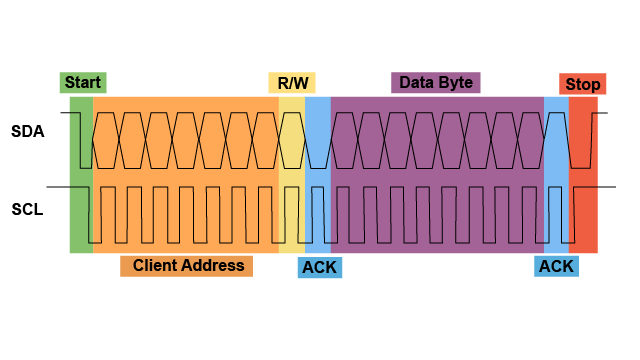
\includegraphics[width=\linewidth]{Figures/i2c-packet.png}
	\caption[Paquet I2C]{Paquet I2C.}
	\label{fig:i2c-packet}
\end{figure}

\section{Calcul de l'orientation}

\paragraph{Il existe plusieurs méthodes pour calculer l'orientation d'un objet à partir des données d'un IMU. Les méthodes les plus courantes sont les filtres de Kalman, les filtres de Mahony et les filtres de Madgwick. Ces filtres utilisent les données de l'accéléromètre, du gyroscope (et du magnétomètre facultatif mais reduit la marge de l'erreur) pour estimer l'orientation de l'objet en temps réel.}

% \paragraph{Le problème de l'estimation de l'orientation à partir des données d'un IMU est la sensibilité au bruit du capteur et aux erreurs de mesure. Les filtres de Kalman, les filtres de Mahony et les filtres de Madgwick sont conçus pour réduire le bruit et les erreurs de mesure en utilisant des modèles mathématiques pour estimer l'orientation de l'objet.}

\subsubsection{Les Angles d'Euler}

\paragraph{Les angles d'Euler sont une méthode courante pour représenter l'orientation d'un objet dans l'espace tridimensionnel. Les angles d'Euler sont composés de trois angles : l'angle de roulis, l'angle de tangage et l'angle de lacet. Ces angles décrivent la rotation de l'objet autour de ses axes X, Y et Z respectivement d'un système de coordonnées fixe.}


\begin{enumerate}
	\item \textbf{Roulis (Roll) :} Rotation autour de l'axe X. $\theta$.
	\item \textbf{Tangage (Pitch) :} Rotation autour de l'axe Y. $\phi$.
	\item \textbf{Lacet (Yaw) :} Rotation autour de l'axe Z. $\psi$.
\end{enumerate}

\begin{equation*}
	R_x = \begin{bmatrix}
		1 & 0 & 0 \\
		0 & \cos(\theta) & -\sin(\theta) \\
		0 & \sin(\theta) & \cos(\theta)
	\end{bmatrix}
\end{equation*}

\begin{equation*}
	R_y = \begin{bmatrix}
		\cos(\phi) & 0 & \sin(\phi) \\
		0 & 1 & 0 \\
		-\sin(\phi) & 0 & \cos(\phi)
	\end{bmatrix}
\end{equation*}

\begin{equation*}
	R_z = \begin{bmatrix}
		\cos(\psi) & -\sin(\psi) & 0 \\
		\sin(\psi) & \cos(\psi) & 0 \\
		0 & 0 & 1
	\end{bmatrix}
\end{equation*}

\begin{equation*}
	R_{xyz} = R_x(\theta) \times R_y(\phi) \times R_z(\psi)
\end{equation*}

\begin{equation*}
	R_{xyz} = \begin{bmatrix}
		\cos(\phi) \cos(\psi) & \cos(\phi) \sin(\psi) & -\sin(\phi) \\
		\sin(\theta) \sin(\phi) \cos(\psi) - \cos(\theta) \sin(\psi) & \sin(\theta) \sin(\phi) \sin(\psi) + \cos(\theta) \cos(\psi) & \sin(\theta) \cos(\phi) \\
		\cos(\theta) \sin(\phi) \cos(\psi) + \sin(\theta) \sin(\psi) & \cos(\theta) \sin(\phi) \sin(\psi) - \sin(\theta) \cos(\psi) & \cos(\theta) \cos(\phi)
	\end{bmatrix}
\end{equation*}

\paragraph{On définit la matrice de R de rotation du capteur par rapport au repère fixe.}

\begin{equation}
	R = R_{xyz}
\end{equation}

% \paragraph{Pour ce projet notre bras posede un seul degré de liberté, donc nous allons utiliser l'angle de roulis pour déterminer la position du bras.}


\subsection{Accéléromètre}

% \paragraph*{On peut estimer l'angle de roulis à partir des données de l'accéléromètre en utilisant l'angle d'inclinaison. L'angle d'inclinaison est l'angle entre l'accélération gravitationnelle et l'axe X de l'objet.}

\subsubsection{Modèle Mathématique}

\paragraph{L'accélération gravitationnelle est définie comme :}

\begin{equation}
	g = 9.81 \, m/s^2
\end{equation}

\paragraph{L'accélération linéaire mesurée par l'accéléromètre est composée de l'accélération gravitationnelle et de l'accélération linéaire de l'objet.}

\begin{equation}
	\vec{a} = \frac{\vec{dv}}{dt} - R * \vec{g} + b_a(t) + n_a(t)
\end{equation}

\begin{enumerate}
	\item $\vec{a}$ est l'accélération linéaire mesurée par l'accéléromètre.
	\item $R$ est la matrice de rotation du capteur.
	\item $b_a(t)$ est le biais de l'accéléromètre.
	\item $n_a(t)$ est le bruit de l'accéléromètre.
\end{enumerate}

\paragraph{Dans un premier temps on se pose au repos donc l'accélération linéaire est nulle aussi nous allons négliger le bruit et le biais de l'accéléromètre pour simplifier le modèle.}

\begin{equation*}
	\vec{a} = -R * \vec{g}
\end{equation*}

\paragraph{On deduit trois equations pour les trois axes de l'accéléromètre.}

\begin{align*}
	a_x &= -g \sin(\theta) \\
	a_y &= g \cos(\theta) \sin(\phi) \\
	a_z &= g \cos(\theta) \cos(\phi)
\end{align*}

\begin{equation}
	\theta(n) = \arcsin\left(\frac{a_x(n)}{g}\right)
\end{equation}

\subsection{Gyroscope}

\paragraph{L'intégrale de la rotation est une méthode simple pour estimer l'orientation d'un objet à partir des données d'un gyroscope. L'intégrale de la rotation consiste à intégrer les données du gyroscope pour estimer l'orientation de l'objet en temps réel.}

\begin{equation}
	\theta(n) = \theta(n - 1) + \omega_x(n) \times \Delta t \\
\end{equation}

\paragraph{Où $\theta(n)$ est l'angle de roulis à l'instant n, $\theta(n - 1)$ est l'angle de roulis à l'instant n-1, $\omega_x$ est la vitesse angulaire autour de l'axe X et $\Delta t$ est l'intervalle de temps entre les mesures.}
